\chapter{回到起点之后：关键帧与位姿图}
\begin{notebox}
\textbf{目标}\quad 用相对运动约束共同调整轨迹，并按新位姿重建观测地图。\\
\textbf{先修}\quad 第 02、08、09 章的坐标变换、最小二乘和传感器融合。
\end{notebox}

\section{从一条链变成一张图}
机器人逐帧估计运动，微小误差会随路程积累。走一圈回到熟悉的墙角时，
里程计的终点可能偏离起点。此时旧扫描和新扫描提供了额外信息：
这两个时刻其实看到了同一个地点，它们的相对位置可以再测一次。
这条跨越很长时间的约束称为\textbf{回环边}。

先运行一个可以直接指定相对位姿的实验：
\begin{lstlisting}[language=bash]
ros2 run motion2d pose_graph_demo tmp/ch10_graph
/usr/bin/python3 scripts/plot_ch10_graph.py
\end{lstlisting}
81 个节点沿 $4\times3$ m 矩形行走，每条相邻节点之间的测量都带有小误差。
把这些测量依次复合，得到逐渐漂移的链。最后加入“末帧与首帧重合”的测量，
优化器就会让所有节点共同调整。本章先弄清这个调整过程，再从实际扫描中寻找回环。

\subsection{先手算只有三个位置的图}
为了看清“共同调整”，暂时只考虑一维。固定 $x_0=0$，
顺序测量是 $x_1-x_0\approx1$ m、$x_2-x_1\approx1$ m，
额外测量却说 $x_2-x_0\approx1.8$ m。
三条边不能同时精确满足；令每条边采用相同的尺度，最小化残差平方和：
\begin{equation}
C(x_1,x_2)=\tfrac12[(x_1-1)^2+(x_2-x_1-1)^2+(x_2-1.8)^2].
\end{equation}
分别求偏导，注意第二项中 $x_1$ 的系数为 $-1$：
\begin{align}
\frac{\partial C}{\partial x_1}&=(x_1-1)-(x_2-x_1-1)=2x_1-x_2=0,\\
\frac{\partial C}{\partial x_2}&=(x_2-x_1-1)+(x_2-1.8)=-x_1+2x_2-2.8=0.
\end{align}
第一式给出 $x_2=2x_1$，代入第二式得到 $x_1=.9333$ m、$x_2=1.8667$ m。
三个残差分别约为 $-.0667,-.0667,+.0667$ m：新增测量与原来的两个测量各分担了一部分误差。

\begin{center}
\begin{tikzpicture}[x=1cm,y=1cm,>=Stealth,
  pose/.style={circle,draw=navy,fill=pale,minimum size=8mm}]
\node[pose,rectangle] (a) at (0,0) {$x_0$};
\node[pose] (b) at (4,0) {$x_1$};
\node[pose] (c) at (8,0) {$x_2$};
\draw[->,thick] (a)--node[above]{测得 $1$ m}(b);
\draw[->,thick] (b)--node[above]{测得 $1$ m}(c);
\draw[->,tealblue,thick] (a.south) to[out=-55,in=-125] node[below]{额外测得 $1.8$ m} (c.south);
\node[above=7mm] at (a) {固定 $0$};
\node[above=7mm] at (b) {$1\ \to\ .9333$};
\node[above=7mm] at (c) {$2\ \to\ 1.8667$};
\end{tikzpicture}
\end{center}
图中的位置变量可以换成二维位姿，边也可以带不同的可信程度。
接下来的计算就是把这个小例子推广到位置与航向一起变化的情况。

\section{二维边残差：比较预测与测量}
每个节点保存关键帧在 map 中的位姿 $T_i=(R_i,p_i)$，
它把帧 $i$ 中的点变到 map。边测量 $Z_{ij}=(R_z,z_{ij})$ 把帧 $j$ 的点变到帧 $i$。
由第二章的逆变换与复合规则，当前节点预测的相对变换为
\begin{equation}
T_i^{-1}T_j=(R_i^\top R_j,\ q),\qquad q=R_i^\top(p_j-p_i).
\end{equation}
$q$ 是“站在第 $i$ 帧看，第 $j$ 帧原点在哪里”。
若预测与测量一致，$Z_{ij}^{-1}T_i^{-1}T_j$ 就等于单位变换。
再做一次复合，得到误差变换的平移与角度：
\begin{equation}
e_{ij}=\begin{bmatrix}R_z^\top(q-z_{ij})\\
\operatorname{wrap}(\psi_j-\psi_i-\psi_{ij})\end{bmatrix}.
\end{equation}
前两项先在 $i$ 帧中相减，再旋转到测量所定义的 $j$ 帧方向；最后一项比较相对航向。
本章直接用这三个数度量误差，所需运算都是二维旋转、平移和角度归一化。

例如 $p_i=(1,2)$ m、$\psi_i=90^\circ$，$p_j=(1,4)$ m、$\psi_j=90^\circ$，
则 $q=R(-90^\circ)(0,2)=(2,0)$ m，相对航向为零。
当测量也为 $z_{ij}=(2,0)$ m、$\psi_{ij}=0$ 时，残差为零。
如果只把 $p_j$ 的全局 $x$ 增加 $.1$ m，$q$ 变成 $(2,-.1)$ m，残差为 $(0,-.1,0)$。
全局向右的小误差，在朝向北的 $i$ 帧中表现为向右侧，即局部 $y$ 负方向。

\subsection{把米和弧度换成统一的误差尺度}
给残差三个方向指定标准差 $\sigma_x,\sigma_y,\sigma_\psi$，分别除以标准差：
\begin{equation}
D_{ij}=\operatorname{diag}(1/\sigma_x,1/\sigma_y,1/\sigma_\psi),\qquad
\widetilde e_{ij}=D_{ij}e_{ij}.
\end{equation}
每个新分量表示偏离了多少个标准差，已经没有单位。这个操作称为白化，
这里采用三个方向相互独立的测量尺度；它们对应上式残差所在的坐标方向。
例如残差 $(.06,0,.04)$、尺度 $(.03,.03,.02)$，得到 $(2,0,2)$，
平方代价为 $\tfrac12(2^2+0^2+2^2)=4$。
尺度减半时，相同误差的平方代价变为四倍，所以该约束会更强地影响轨迹。

顺序边使用 $\tfrac12\|\widetilde e\|^2$；回环边对范数使用第八章的 Huber 损失，
默认阈值为 3。它让很大的回环残差以线性速度增加代价，降低单条异常边对整张图的拉动。

\section{固定第一帧，就是给地图选坐标原点}
只有相对测量时，把整张图平移或转动都不会改变测量预测。
设所有位姿同时左乘固定变换 $A$，利用 $(AT_i)^{-1}=T_i^{-1}A^{-1}$，有
\begin{equation}
(AT_i)^{-1}(AT_j)=T_i^{-1}A^{-1}AT_j=T_i^{-1}T_j.
\end{equation}
也就是说，同一组相对残差对应无数张整体位置和朝向不同的图。
在最小二乘方程里，这表现为有些增量方向不会改变代价，因而解不唯一。
一维小例子若连 $x_0$ 也一起优化，给三个 $x$ 同时加任意常数就会发生这种情况。

固定首帧的 $x,y,\psi$ 后，地图的三个整体自由度就确定了。
代码把节点 0 留在原处，只把节点 $1,\ldots,N-1$ 的三个数写进优化变量，
总维数为 $3(N-1)$。首帧数值来自坐标原点的选择，可以取零，也可以取其他给定位置。
若图包含互不连接的两部分，第二部分仍可自行平移旋转，
因此程序用图遍历检查所有节点能否从首帧到达，并以 \code{disconnected} 提示缺少连接约束。

\section{对一条边的两端分别求导}
采用加法更新 $p_i\leftarrow p_i+\delta p_i$、$\psi_i\leftarrow\psi_i+\delta\psi_i$。
记 $J=\left[\begin{smallmatrix}0&-1\\1&0\end{smallmatrix}\right]$。
由 $q=R_i^\top(p_j-p_i)$ 直接得到
\begin{equation}
\frac{\partial q}{\partial p_i}=-R_i^\top,\quad
\frac{\partial q}{\partial p_j}=R_i^\top,\quad
\frac{\partial q}{\partial\psi_i}=-Jq,\quad
\frac{\partial q}{\partial\psi_j}=0.
\end{equation}
第三项可从 $R_i^\top=R(-\psi_i)$ 看出：对 $\psi_i$ 求导为 $-JR_i^\top$，再乘位置差。
第四项为零，是因为改变末帧的朝向并不改变它的原点位置。
测量 $R_z,z_{ij}$ 在求导时保持不变，因此 $e_p=R_z^\top(q-z_{ij})$ 的每一块偏导
只需在左边再乘 $R_z^\top$。角度残差对两端航向的导数分别为 $-1,+1$，于是
\begin{align}
A_{ij}=\frac{\partial e}{\partial(p_i,\psi_i)}
&=\begin{bmatrix}-R_z^\top R_i^\top&-R_z^\top Jq\\0\;0&-1\end{bmatrix},\\
B_{ij}=\frac{\partial e}{\partial(p_j,\psi_j)}
&=\begin{bmatrix}R_z^\top R_i^\top&0\\0\;0&1\end{bmatrix}.
\end{align}
例如 $R_i=R_z=I$、$q=(2,1)$ m，则
\begin{equation}
A=\begin{bmatrix}-1&0&1\\0&-1&-2\\0&0&-1\end{bmatrix},\qquad B=I.
\end{equation}
只增加起点航向 $.01$ rad，预测残差约变化 $(.01,-.02,-.01)$。
可以用这个数值例子核对源码的 \code{q.y(), -q.x()} 符号。
航向残差跨越 $\pm\pi$ 时先归一化；中心差分的两次扰动应落在同一角度分支内，检验局部导数。

\par\noindent\begin{minipage}{\linewidth}
\lstinputlisting[language=C++,linerange={graph_residual_begin-graph_residual_end},
  includerangemarker=false]{../ros2_ws/src/motion2d/src/estimation/pose_graph.cpp}
\end{minipage}\par

\section{把许多小方程装成一个大方程}
一条边只依赖两端节点。将白化雅可比记为 $J_i=DA$、$J_j=DB$，
一阶近似为 $\widetilde e(\delta)\approx\widetilde e+J_i\delta_i+J_j\delta_j$。
第八章已从残差平方和推得 $H\delta=-g$。现在对这一条边展开二次代价，
与两端有关的贡献恰好是
\begin{equation}
\begin{bmatrix}H_{ii}&H_{ij}\\H_{ji}&H_{jj}\end{bmatrix}
\mathrel{+}=w\begin{bmatrix}J_i^\top J_i&J_i^\top J_j\\
J_j^\top J_i&J_j^\top J_j\end{bmatrix},\qquad
\begin{bmatrix}g_i\\g_j\end{bmatrix}\mathrel{+}=w\begin{bmatrix}J_i^\top\widetilde e\\J_j^\top\widetilde e\end{bmatrix}.
\end{equation}
$\mathrel{+}=$ 表示把本条边的贡献加到已有数值上。
普通边 $w=1$；由第八章的 Huber 导数得到回环权重
$w=\min(1,3/\|\widetilde e\|)$，零残差时取 1。
每个 $H_{ij}$ 都是 $3\times3$ 小块，没有边相连的节点对不会直接贡献块。
因此尽管图有很多节点，矩阵中仍有大量零，称为\textbf{稀疏矩阵}。

节点 $k\geq1$ 对应大向量从 $3(k-1)$ 开始的三个位置。
下面代码对一条边的两个端点分别遍历，跳过固定节点，把四个小块按行列位置装进去。
\code{Triplet} 存储“行、列、值”；\code{setFromTriplets} 会把落在同一位置的值相加。

\par\noindent\begin{minipage}{\linewidth}
\lstinputlisting[language=C++,linerange={graph_assembly_begin-graph_assembly_end},
  includerangemarker=false]{../ros2_ws/src/motion2d/src/estimation/pose_graph.cpp}
\end{minipage}\par

在三个位置的一维例子中，收集各边偏导可得
$H=\left[\begin{smallmatrix}2&-1\\-1&2\end{smallmatrix}\right]$。
在初值 $(x_1,x_2)=(1,2)$ 处，$g=(0,.2)^\top$。
解 $H\delta=-g$ 得 $\delta=(-.0667,-.1333)^\top$，正好得到本章开头的答案。
二维问题的旋转是非线性的，所以更新后要重新计算残差和雅可比，再求下一步。

\subsection{为什么有时只走半步}
一阶近似在增量较小时更可靠。求出 $\delta$ 后，先尝试完整增量，
若实际代价下降不够，再尝试 $\delta/2,\delta/4,\ldots$，称为回溯线搜索。
设当前总代价为 $C$，沿增量方向的一阶变化率是 $g^\top\delta$。
因为 $H\delta=-g$，正定时
$g^\top\delta=-\delta^\top H\delta<0$，这是一个下降方向。
代码用条件
\begin{equation}
C(x+\alpha\delta)\leq C(x)+10^{-4}\alpha g^\top\delta
\end{equation}
要求实际下降达到一阶预测下降量的一小部分，并依次尝试 $\alpha=1,1/2,\ldots,1/1024$。
所有增量分量都很小时报告收敛；若方程奇异、迭代耗尽或所有步长都被拒绝，
保留当前图并返回对应状态，便于检查初值和边约束。

\subsection{错误回环为何仍需先做几何检查}
考虑一个位置 $x$，正常测量为 1 m，错误回环测量为 10 m，两者标准差均为 $.1$ m。
普通平方代价的导数是 $100(x-1)+100(x-10)$，令其为零得到 $x=5.5$ m。
若只对回环用阈值 3 的 Huber，在 $x$ 接近 1 时，回环白化残差为 $10(x-10)<-3$，
Huber 对它的导数为 $-3$，再乘链式因子 10，得到对 $x$ 的导数 $-30$。
总导数于是变成 $100(x-1)-30$，最优位置为 $x=1.3$ m，且满足所用的线性分支条件。
鲁棒损失把错误回环的拉力限制住了，仍然留下 $.3$ m 偏移。
所以回环进入图之前，还需要检查两帧点云是否重叠、配准是否稳定和往返变换是否一致。

\clearpage
\section{矩形实验与可独立检验的答案}
固定 seed=1010，沿四条边各走 20 步。每步加独立 $0.01$ m 平移噪声、$0.002$ rad 航向噪声，
并注入每步 $0.003$ rad 航向偏差。顺序边的测量尺度为 $(.03,.03,.02)$；
闭环观测为单位变换，尺度 $(.02,.02,.01)$。参考轨迹仅用于评估，不送给优化器。
\begin{figure}[h]
\centering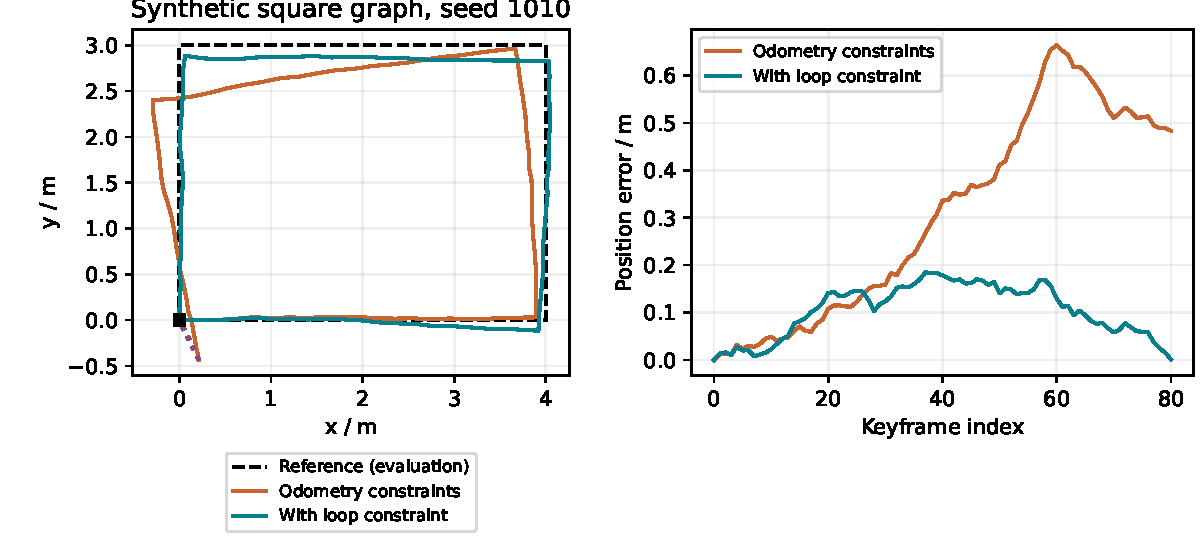
\includegraphics[width=\linewidth]{figures/ch10_graph.pdf}
\caption{合成位姿图的优化前后结果。左图等比例，方块为固定首帧，紫色虚线指出原始链的闭合缺口。}
\end{figure}
\begin{center}\small
\pgfplotstabletypeset[col sep=comma,
columns={mode,position_rmse,closure_error,final_cost,iterations},
columns/mode/.style={column name=约束,string type,string replace*={odometry}{顺序边},string replace*={loop}{加回环}},
columns/position_rmse/.style={column name=位置 RMSE/m,fixed,precision=4},
columns/closure_error/.style={column name=闭合误差/m,fixed,precision=4},
columns/final_cost/.style={column name=最终代价,fixed,precision=4},
columns/iterations/.style={column name=迭代},
every head row/.style={before row=\toprule,after row=\midrule},
every last row/.style={after row=\bottomrule}]{data/ch10_graph.csv}
\end{center}
顺序边代价几乎为零，因为链本身就是由这些边累乘出来的：每个相邻位姿都精确满足带误差的测量。
加入新约束后边之间有冲突，最优代价可以大于零，而参考误差反而下降。
因此，代价衡量图内约束的吻合程度，位置 RMSE 则衡量相对于参考轨迹的误差；应结合两者解释结果。

\textbf{练习 ch10-1：}补完 edge\_residual.hpp，检查旋转坐标和角度跨界。
理解题证明左乘不变性；实验题改变回环尺度，比较全程 RMSE、闭合误差、代价与求解状态。
常见错误包括变换乘法顺序颠倒、只锚定位置却漏掉航向、把错误闭环交给鲁棒核“自动判断”。

\textbf{手算练习：}在三节点例子中将额外边的标准差减半。
这相当于把它的平方项乘以 4；重新求两个偏导为零的方程，观察误差如何重新分配。

\clearpage
\section{从关键帧中寻找旧地点}
完整管线沿用第九章前端；后端只接收扫描及同一采样时刻的校正位姿。
平移达到 0.3 m、航向变化达到 0.25 rad，或距上帧达到 2 s，就保存一个关键帧。
其中既有原始距离数组，也有机体系的体素点云和局部法向量。
机体系观测保留了采样时的原始几何，后面改变关键帧的全局位姿时，可用它重新投影地图。

\begin{lstlisting}[language=bash]
ros2 launch motion2d_bringup ch10.launch.py rviz:=false
# Another terminal, same ROS environment, repository root:
/usr/bin/python3 scripts/check_ch10.py
\end{lstlisting}
排除最近 20 个关键帧后，只在当前估计位置的 0.8 m 范围内寻找候选，航向差小于 0.6 rad。
每次最多检查距离最近的三个候选。候选搜索以当前估计为中心，适合累计漂移仍小于搜索半径的场景。漂移超过半径时，旧地点会落在窗口之外；扩大窗口能找回更多候选，也会增加误匹配的机会。
成功回环后至少等待五个新关键帧，避免高频重复加入同一个地点的相关证据。

\begin{center}\small
\begin{tabular}{ll}\toprule
几何检查 & 默认条件 \\\midrule
双向点到线 ICP & 两个方向都收敛，且没有秩退化 \\
有效对应比例 & 两个方向均至少 $55\%$ \\
残差与初值偏离 & RMSE 不超过 0.05 m；校正不超过 0.5 m / 0.25 rad \\
往返一致性 & 平移不超过 0.03 m，航向不超过 0.02 rad \\\bottomrule
\end{tabular}
\end{center}
若正向变换为 $T_{ij}$，反向为 $T_{ji}$，则一致时 $T_{ij}T_{ji}\approx I$。
将正向变换写成 $(R_f,t_f)$、反向变换写成 $(R_b,t_b)$，复合后的平移为
$t_f+R_ft_b$，角度为 $\operatorname{wrap}(\psi_f+\psi_b)$。
例如正向平移 $(1,0)$ m、转 $90^\circ$，反向应平移 $(0,1)$ m、转 $-90^\circ$；
因为 $R(90^\circ)(0,1)=(-1,0)$，往返平移才会相消。
下面代码按这个复合公式检查；通过各项门限后才生成回环边。
\lstinputlisting[language=C++,linerange={loop_cycle_begin-loop_cycle_end},
  includerangemarker=false]{../ros2_ws/src/motion2d/src/estimation/loop_closure.cpp}

平行长墙沿墙方向缺少约束，可由第八章的秩检查识别。
重复房间则可能在两个方向都得到相似的点云：即使往返变换很小，仍需结合更长时间的运动历史
或更有辨识度的场景特征区分地点。可以主动构造这两种场景，分别观察退化拒绝和地点混淆。
图优化失败时撤掉新回环边，继续使用已有的局部里程计和顺序边。

当前最多保留 200 个关键帧，达到容量后以 \code{capacity_reached} 提示停止加入新帧。
关键帧越多，逐帧重建地图的计算量也越大；更大场景可将若干关键帧组成子图，按子图组织更新。

\clearpage
\section{回环更新地图坐标，不改写局部里程计}
同一机器人有局部位姿 $T_{OB}$ 和图优化后的全局位姿 $T_{MB}$，满足
\begin{equation}
T_{MB}=T_{MO}T_{OB},\qquad T_{MO}=T_{MB}T_{OB}^{-1}.
\end{equation}
第二式由第一式在右边乘 $T_{OB}^{-1}$ 得到。展开为旋转和平移，就是
\begin{equation}
R_{MO}=R_{MB}R_{OB}^\top,\qquad
p_{MO}=p_{MB}-R_{MO}p_{OB}.
\end{equation}
例如同一关键帧的全局位姿为 $p_{MB}=(10,-2)$ m、$\psi_{MB}=180^\circ$，
局部位姿为 $p_{OB}=(2,1)$ m、$\psi_{OB}=90^\circ$。
则校正旋转为 $90^\circ$，先算 $R_{MO}p_{OB}=(-1,2)$，再相减得到 $p_{MO}=(11,-4)$ m。
将其代回 $p_{MB}=p_{MO}+R_{MO}p_{OB}$，即可核对 $(10,-2)$。
程序用最新关键帧的两种位姿计算这个校正，原始 odom 位姿继续保存自己的运动历史。
\textbf{练习 ch10-2} 完成 map\_alignment.hpp，先手算带 $90^\circ$ 旋转的例子。
仅把两个位置相减会漏掉旋转，无法得到正确变换。

\lstinputlisting[language=C++,linerange={map_alignment_begin-map_alignment_end},
  includerangemarker=false]{../ros2_ws/src/motion2d/src/estimation/keyframes.cpp}

一条 TF 边只有一个发布者：SLAM 发布 map 到 odom；estimated 适配器发布 odom 到 base\_link；
模拟器只保留圆心处传感器的静态外参。回环可以让机器人在 map 中跳到更一致的位置，
但不会把这个全局位移直接写入局部运动链。第十九章会处理全局目标与局部控制参考的衔接。

\begin{center}\small
\begin{tabular}{ll}\toprule
输出 & 含义 \\\midrule
\texttt{/map/cloud} 与 \texttt{/map} & 按最新图位姿重建的点云与观测栅格 \\
\texttt{/path/graph\_before} & 固定首帧基准中的原始里程计关键帧 \\
\texttt{/path/graph\_after} & 同一基准中的优化关键帧 \\
\texttt{/slam/edges} & 顺序边与紫色回环边 \\
\texttt{/slam/status} & 更新/拒绝状态及关键帧、回环计数 \\\bottomrule
\end{tabular}
\end{center}
前后路径都用首帧固定的 map 基准比较，不再用当前 map 到 odom 把原始基线变换第二次。
高频局部轨迹仍由第九章输出；图更新频率是关键帧频率。

\textbf{为什么要重建：}设旧图在 $x=3$ m 有一面墙，优化后这次观测应落在 $x=4$ m。
直接追加新点会留下两面墙。重建时新建空栅格，再遍历所有保留的原始扫描，
按照各自优化后的采样位姿重新做射线清空与端点占据；体素点云也重新生成。
本章累积的是关键帧的实际观测，未被光线照到的区域保留未知状态。

只改一条全局 TF，也无法修正不同历史帧之间的相对错位。
设旧点云中两个点为 $u,v$，施加相同刚体变换后，它们的距离仍为
\begin{equation}
\|(Ru+t)-(Rv+t)\|=\|R(u-v)\|=\|u-v\|.
\end{equation}
最后一步使用 $R^\top R=I$：旋转保持长度。
因此要把两次错开的墙面观测重新对齐，就必须分别使用各自优化后的关键帧位姿。

\begin{center}
\begin{tikzpicture}[x=1cm,y=1cm,>=Stealth,
  box/.style={draw=tealblue,fill=pale,rounded corners=2pt,align=center,minimum height=9mm}]
\node[box] (local) at (0,0) {各帧局部扫描};
\node[box] (pose) at (0,-1.6) {各帧优化位姿};
\node[box] (project) at (4,-.8) {逐帧重新投影};
\node[box] (map) at (8,-.8) {新栅格与点云};
\draw[->] (local.east)--(project.north west);
\draw[->] (pose.east)--(project.south west);
\draw[->] (project)--node[above=6mm,font=\small]{重新累积}(map);
\end{tikzpicture}
\end{center}

\clearpage
\section{实际激光与 IMU 的矩形回放}
\begin{lstlisting}[language=bash]
ros2 run motion2d slam_demo tmp/ch10_slam
/usr/bin/python3 scripts/plot_ch10_slam.py
\end{lstlisting}
使用 $14\times12$ m 房间，内部有一个圆与一个三角形。
半径 0.2 m 的全向圆盘沿 $6\times4$ m 矩形行走，每边 6 s，平滑的时间规律让它在拐角静止（第十四章推导这条五次曲线）；
机体 yaw 保持零。四条边均通过整段扫掠检查。
360 束、距离噪声 0.03 m、激光 10 Hz、IMU 200 Hz，噪声 seed=4242/6060。

\begin{figure}[h]
\centering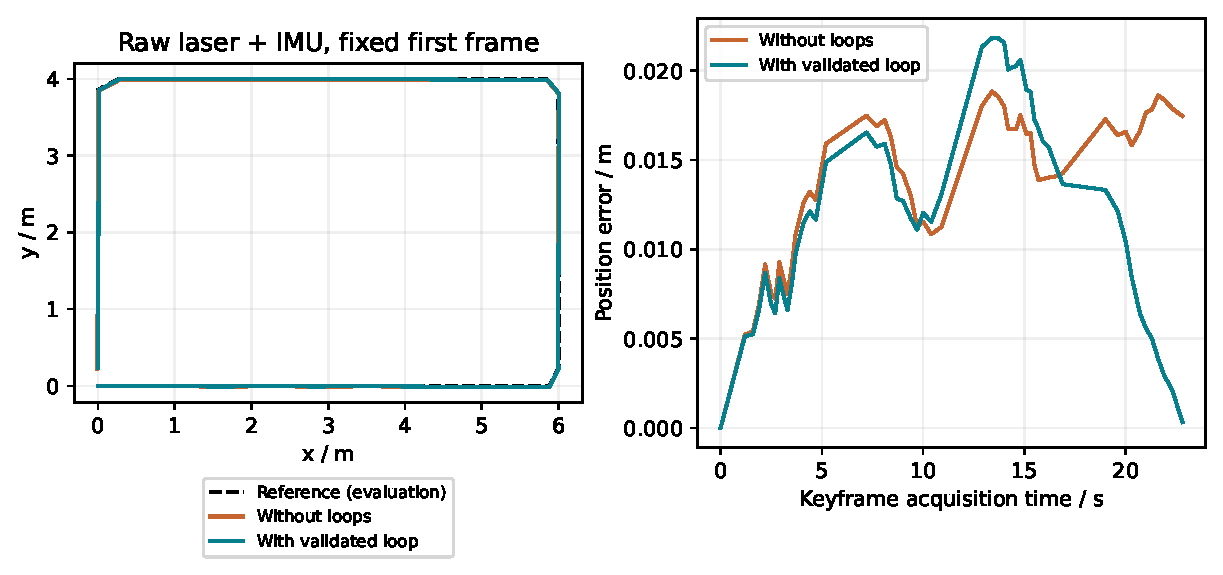
\includegraphics[width=\linewidth]{figures/ch10_slam.pdf}
\caption{同一真实传感器前端输出，分别送给回环关闭和开启的图。误差只统计关键帧；参考轨迹仅用于评估。}
\end{figure}
\begin{center}\small
\pgfplotstabletypeset[col sep=comma,
columns={mode,keyframes,loops,position_rmse,final_position_error},
columns/mode/.style={column name=模式,string type,string replace*={no_loop}{关闭回环},string replace*={loop}{开启回环}},
columns/keyframes/.style={column name=关键帧},columns/loops/.style={column name=回环},
columns/position_rmse/.style={column name=位置 RMSE/m,fixed,precision=4},
columns/final_position_error/.style={column name=末关键帧误差/m,fixed,precision=4},
every head row/.style={before row=\toprule,after row=\midrule},
every last row/.style={after row=\bottomrule}]{data/ch10_slam.csv}
\end{center}
本例在 22.3 s 检查一个候选并接受回环；最后关键帧时间为 22.8 s。
表中的末帧误差取 22.8 s 的关键帧位置与同一时刻参考位置之差；首尾闭合距离则取末帧与首帧之差，两者使用的参照不同。
激光拒绝 27 帧，EKF 无额外拒绝；失败扫描没有进入图。

回环显著改善了靠近返回地点的关键帧，但部分中间点误差反而略增。
全程位置 RMSE 从约 1.44 cm 降至 1.32 cm；末帧误差则从约 1.75 cm 降至 0.033 cm。末帧接近回环约束的位置，因而改善更明显；其他节点还要兼顾沿途顺序边。
所有 CSV、原始地图 PGM 与点云 CSV 均可由上述命令重新生成。

\clearpage
\section{从地图中观察回环的作用}
\begin{figure}[h]
\centering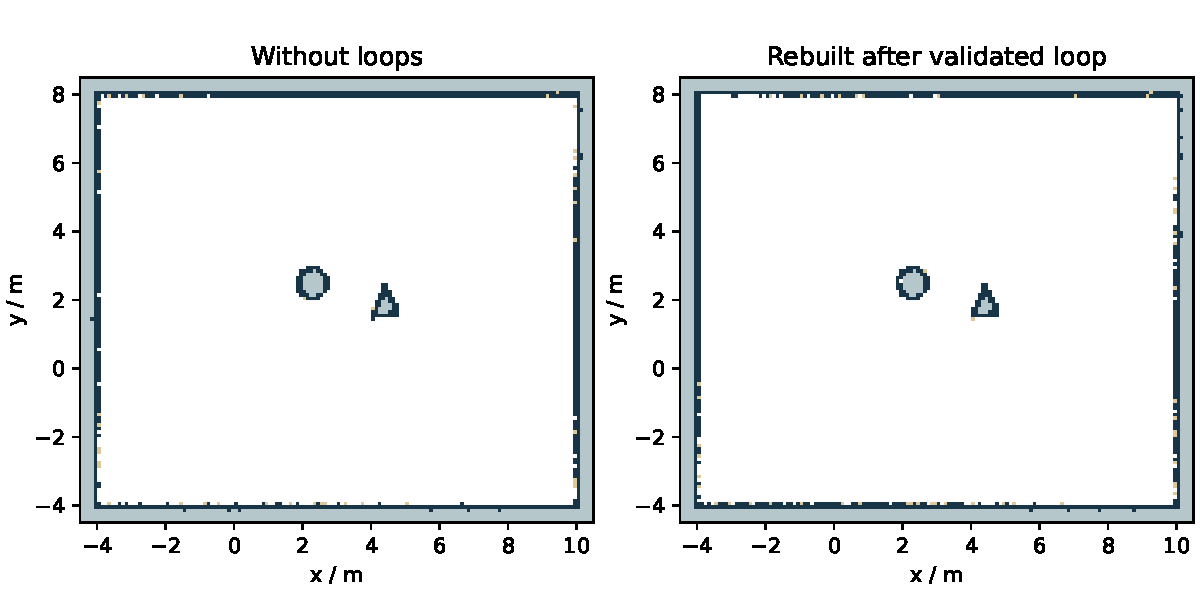
\includegraphics[width=\linewidth]{figures/ch10_maps.pdf}
\caption{两图均由关键帧扫描构建，分辨率 0.1 m。白色自由，深色占据，灰色未知，浅褐色为已观测但不确定；横纵尺度相同。}
\end{figure}
本例原始误差只有厘米量级，小于地图分辨率，因此两张全景图很接近。
可以做一个更容易看清的实验：只把某个关键帧的墙面观测位姿移动一个格子，分别尝试追加与重建。
追加会留下旧墙，重建则根据所有关键帧的新位姿重新决定每个格子的证据。
圆与三角形内部没有被光线穿透，仍然保留未知区域。

启动默认 RViz 配置时，应看到优化关键帧、紫色回环边、重建点云和占据图；
原始世界与真值机器人默认隐藏。可修改配置中的 slam.enable\_loops 为 false 对照。
\begin{enumerate}
\item \textbf{理解：}为什么只有修改 TF、不重建历史点云，会得到坐标正确但几何仍旧扭曲的地图？
\item \textbf{代码：}完成两道练习，检查边残差的变换顺序和 map 到 odom 的计算。
\item \textbf{实验：}改变候选距离、关键帧间隔或激光噪声，记录候选数、接受数、拒绝帧与误差。
\item \textbf{失败：}用单面墙验证退化，用无重叠云验证拒绝；达到图容量时应看到明确状态。
\end{enumerate}

本章将激光/IMU 局部定位、几何回环和地图重建连成了一个小场景 SLAM 系统。
继续扩大场景时，可以研究全局地点识别、动态物体处理及子图管理。
下一章从真值定位和观测地图开始学习路径搜索，再逐步将规划与本章的定位建图结果连接起来。
